% NodeDiffusion architecture — BERT + Cross-Attention version
% Compile: xelatex node_diffusion_arch.tex
\documentclass[tikz, border=14pt]{standalone}
\usepackage{amsmath}
\usepackage{tikz}
\usetikzlibrary{positioning, arrows.meta, fit, backgrounds, calc}

% ── Palette ──────────────────────────────────────────────────────────────────
\definecolor{Ci}{RGB}{207,226,248}   % blue  – inputs / outputs
\definecolor{Ce}{RGB}{250,228,182}   % amber – embedding
\definecolor{Cs}{RGB}{188,220,230}   % steel – encoder
\definecolor{Cp}{RGB}{247,202,202}   % pink  – prediction
\definecolor{Ct}{RGB}{220,240,220}   % green – BERT
\definecolor{Cbdr}{RGB}{148,148,148}

% ── Styles ───────────────────────────────────────────────────────────────────
\tikzset{
  B/.style n args={1}{
    draw=Cbdr, fill=#1, rounded corners=3pt,
    minimum width=2.9cm, minimum height=0.8cm,
    align=center, inner sep=6pt, font=\small\sffamily
  },
  W/.style n args={1}{
    draw=Cbdr, fill=#1, rounded corners=3pt,
    minimum width=6.2cm, minimum height=0.8cm,
    align=center, inner sep=6pt, font=\small\sffamily
  },
  BW/.style n args={1}{
    draw=Cbdr, fill=#1, rounded corners=3pt,
    minimum width=4.4cm, minimum height=0.8cm,
    align=center, inner sep=6pt, font=\small\sffamily
  },
  HW/.style n args={1}{
    draw=Cbdr, fill=#1, rounded corners=3pt,
    minimum width=2.85cm, minimum height=0.8cm,
    align=center, inner sep=4pt, font=\small\sffamily
  },
  C/.style n args={1}{
    circle, draw=Cbdr, fill=#1,
    minimum size=0.58cm, inner sep=0pt, font=\small\sffamily
  },
  grp/.style={draw=Cbdr!55, fill=black!2,
    rounded corners=6pt, line width=0.7pt, dashed},
  ttl/.style={font=\small\sffamily\bfseries, text=black!60},
  a/.style={-{Stealth[length=5pt,width=4pt]},
    line width=0.9pt, color=black!50},
  sk/.style={-{Stealth[length=4pt,width=3pt]},
    line width=0.75pt, color=black!55, dashed}
}

\begin{document}
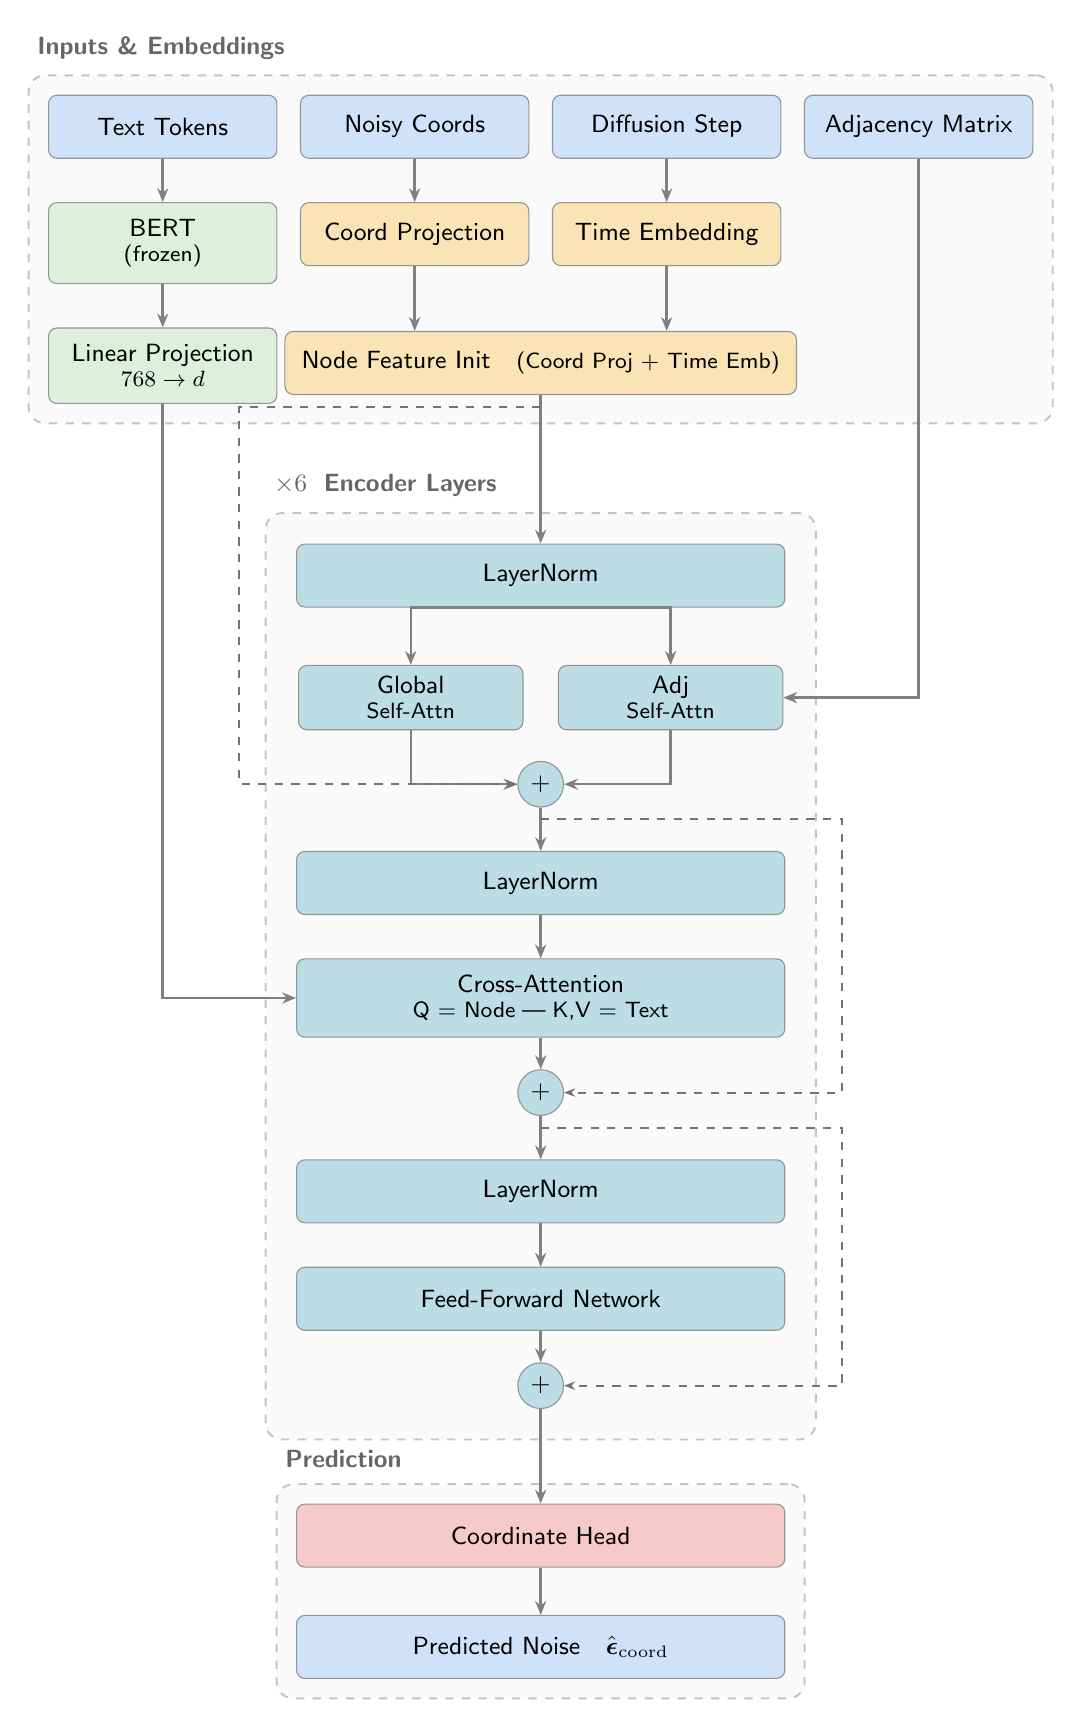
\begin{tikzpicture}

% ─────────────────────────────────────────────────────────────────────────────
%  ROW 0  Raw inputs
% ─────────────────────────────────────────────────────────────────────────────
\node[B={Ci}] (txt) at (-4.8,  0)  {Text Tokens};
\node[B={Ci}] (xin) at (-1.6,  0)  {Noisy Coords};
\node[B={Ci}] (tin) at ( 1.6,  0)  {Diffusion Step};
\node[B={Ci}] (adj) at ( 4.8,  0)  {Adjacency Matrix};

% ─────────────────────────────────────────────────────────────────────────────
%  ROW 1  Text branch: BERT (frozen)
% ─────────────────────────────────────────────────────────────────────────────
\node[B={Ct}, below=0.55cm of txt] (bert)
  {BERT\\[-2pt]\footnotesize(frozen)};

% ─────────────────────────────────────────────────────────────────────────────
%  ROW 1  Node branch: coord proj + time emb
% ─────────────────────────────────────────────────────────────────────────────
\node[B={Ce}, below=0.55cm of xin] (cp)  {Coord Projection};
\node[B={Ce}, below=0.55cm of tin] (tm)  {Time Embedding};

% ─────────────────────────────────────────────────────────────────────────────
%  ROW 2  Text proj  +  Node feature init
% ─────────────────────────────────────────────────────────────────────────────
\node[B={Ct}, below=0.55cm of bert] (tp)
  {Linear Projection\\[-2pt]\footnotesize$768 \to d$};

\node[W={Ce}] (ni) at (0, -3.0)
  {Node Feature Init\quad\footnotesize(Coord Proj $+$ Time Emb)};

% ─────────────────────────────────────────────────────────────────────────────
%  Group: Inputs + Embeddings
% ─────────────────────────────────────────────────────────────────────────────
\begin{scope}[on background layer]
  \node[grp, fit=(txt)(xin)(tin)(adj)(bert)(tp)(cp)(tm)(ni),
        inner sep=7pt] (Ginput) {};
\end{scope}
\node[ttl, anchor=south west] at ([yshift=2pt]Ginput.north west) {Inputs \& Embeddings};

% ─────────────────────────────────────────────────────────────────────────────
%  ENCODER  ×6
%  Sub-layers: (1) Adj Attn + Global Attn (parallel sum)  (2) Cross-Attn  (3) FFN
% ─────────────────────────────────────────────────────────────────────────────
\node[W={Cs}]  (ln1)  at (0, -5.7)  {LayerNorm};

% dual-stream: two narrow boxes side by side (2.85cm each, gap ~0.45cm, total ~6.15cm)
\node[HW={Cs}] (ga) at (-1.65, -7.25) {Global\\[-2pt]\footnotesize Self-Attn};
\node[HW={Cs}] (aa) at ( 1.65, -7.25) {Adj\\[-2pt]\footnotesize Self-Attn};

% single + merges both stream outputs AND residual
\node[C={Cs}]  (add1) at (0, -8.35) {$+$};

\node[W={Cs}, below=0.55cm of add1] (ln2)  {LayerNorm};
\node[W={Cs}, below=0.55cm of ln2]  (ca)
  {Cross-Attention\\[-2pt]\footnotesize Q = Node\;|\;K,V = Text};
\node[C={Cs}, below=0.4cm of ca]    (add2) {$+$};

\node[W={Cs}, below=0.55cm of add2] (ln3)  {LayerNorm};
\node[W={Cs}, below=0.55cm of ln3]  (ffn)  {Feed-Forward Network};
\node[C={Cs}, below=0.4cm of ffn]   (add3) {$+$};

\begin{scope}[on background layer]
  \node[grp, fit=(ln1)(aa)(ga)(add1)(ln2)(ca)(add2)(ln3)(ffn)(add3),
        inner sep=11pt] (Genc) {};
\end{scope}
\node[ttl, anchor=south west] at ([yshift=2pt]Genc.north west)
  {$\times 6$\; Encoder Layers};

% ─────────────────────────────────────────────────────────────────────────────
%  PREDICTION
% ─────────────────────────────────────────────────────────────────────────────
\node[W={Cp}, below=1.2cm of add3] (head)
  {Coordinate Head};
\node[W={Ci}, below=0.6cm of head] (out)
  {Predicted Noise\quad$\hat{\boldsymbol{\epsilon}}_{\mathrm{coord}}$};

\begin{scope}[on background layer]
  \node[grp, fit=(head)(out), inner sep=7pt] (Gpred) {};
\end{scope}
\node[ttl, anchor=south west] at ([yshift=2pt]Gpred.north west) {Prediction};

% ─────────────────────────────────────────────────────────────────────────────
%  ARROWS
% ─────────────────────────────────────────────────────────────────────────────

% inputs → projections
\draw[a] (txt) -- (bert);
\draw[a] (xin) -- (cp);
\draw[a] (tin) -- (tm);
\draw[a] (bert) -- (tp);

% coord proj + time emb → node feature init
\draw[a] (cp.south) -- (cp.south |- ni.north);
\draw[a] (tm.south) -- (tm.south |- ni.north);

% node init → ln1
\draw[a] (ni.south) -- (ln1.north);

% ln1 → fork → adj and global
\draw[a] (ln1.south) -| (aa.north);
\draw[a] (ln1.south) -| (ga.north);

% adj and global outputs → add1
\draw[a] (aa.south) |- (add1.east);
\draw[a] (ga.south) |- (add1.west);

% residual skip 1: ni bypasses ln1+dual-stream to add1
\draw[sk]
  let \p1=(ni.south), \p2=(add1.west), \p3=(Genc.west) in
  (\x1, \y1-0.15cm)
  -- (\x3-0.32cm, \y1-0.15cm)
  -- (\x3-0.32cm, \y2)
  -- (\x2, \y2);

% add1 → ln2 → cross-attn → add2
\draw[a] (add1.south) -- (ln2.north);
\draw[a] (ln2.south)  -- (ca.north);
\draw[a] (ca.south)   -- (add2.north);

% text features → cross-attn from left
\draw[a] (tp.south) |- ([yshift=0.0cm]ca.west);

% adjacency → adj self-attn from right
\draw[a]
  (adj.south)
  -- (adj.south |- aa.east)
  -- (aa.east);

% residual skip 2: add1 bypasses ln2+ca to add2
\draw[sk]
  let \p1=(add1.south), \p2=(add2.east), \p3=(Genc.east) in
  (\x1, \y1-0.15cm)
  -- (\x3+0.32cm, \y1-0.15cm)
  -- (\x3+0.32cm, \y2)
  -- (\x2, \y2);

% add2 → ln3 → ffn → add3
\draw[a] (add2.south) -- (ln3.north);
\draw[a] (ln3.south)  -- (ffn.north);
\draw[a] (ffn.south)  -- (add3.north);

% residual skip 3: add2 bypasses ln3+ffn to add3
\draw[sk]
  let \p1=(add2.south), \p2=(add3.east), \p3=(Genc.east) in
  (\x1, \y1-0.15cm)
  -- (\x3+0.32cm, \y1-0.15cm)
  -- (\x3+0.32cm, \y2)
  -- (\x2, \y2);

% encoder → prediction
\draw[a] (add3.south) -- (head.north);
\draw[a] (head.south) -- (out.north);

\end{tikzpicture}
\end{document}
